% (c) 2012 -2014 Dimitrios Vrettos - d.vrettos@gmail.com

\section{Esercizi}
\subsection{Esercizi dei singoli paragrafi}
\subsubsection*{18.1 - Intervalli sulla retta reale}

\begin{esercizio}
 \label{ese:18.1}
 Determina la scrittura corretta per il seguente grafico.
 \begin{center}
  % (c) 2012 Dimitrios Vrettos - d.vrettos@gmail.com
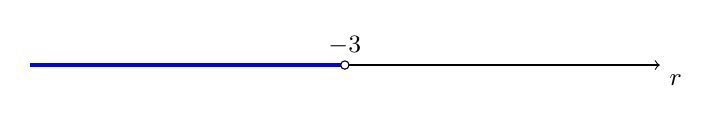
\begin{tikzpicture}[font=\small,x=10mm, y=5mm]

\draw[->] (0,0) -- (8,0) node [below right] () {$r$};
\node[above]  at (4,0) {$-3$};
\begin{scope}[blue,ultra thick]
\draw (0,0) -- (4,0);
\end{scope}
\draw[fill=white] (4,0)circle (1.5pt);

\end{tikzpicture}

 \boxA\quad~$x<-3$ \quad\boxB\quad~$x>-3$\quad\boxC\quad~$x\le -3$\quad\boxD\quad~$x\le -3$
 \end{center}

\end{esercizio}

\begin{esercizio}
 \label{ese:18.2}
 Determina la scrittura corretta per il seguente grafico.
  \begin{center}
  % (c) 2012 Dimitrios Vrettos - d.vrettos@gmail.com
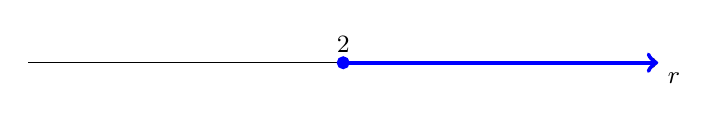
\begin{tikzpicture}[font=\small,x=10mm, y=5mm]

\draw[->] (0,0) -- (8,0) node [below right] () {$r$};
\node[above]  at (4,0) {$2$};
\begin{scope}[blue,ultra thick,->]
\draw (4,0) -- (8,0);
\draw[fill=blue] (4,0)circle (1.5pt);
\end{scope}

\end{tikzpicture}

\boxA\quad~$x<2$\quad\boxB\quad~$x>2$\quad\boxC\quad~$x\ge~2$\quad\boxD\quad~$x\le~2$
 \end{center}
\end{esercizio}

\begin{esercizio}
 \label{ese:18.3}
 Determina la scrittura corretta per il seguente grafico.
  \begin{center}
  % (c) 2012 Dimitrios Vrettos - d.vrettos@gmail.com
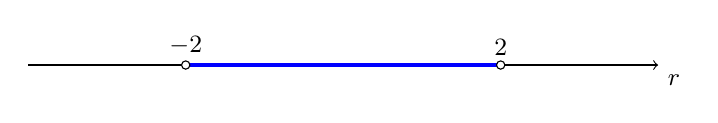
\begin{tikzpicture}[font=\small,x=10mm, y=5mm]

\draw[->] (0,0) -- (8,0) node [below right] () {$r$};
\node[above]  at (2,0) {$-2$};
\node[above]  at (6,0) {2};
\begin{scope}[blue,ultra thick]
\draw (2,0) -- (6,0);
\end{scope}
\foreach \x in {2,6}
\draw[fill=white] (\x,0)circle (1.5pt);

\end{tikzpicture}

\boxA\quad~$x<+2$\quad\boxB\quad~$x>-2$\quad\boxC\quad~$-2\le x\le~2$\quad\boxD\quad~$-2<x<2$
 \end{center}
\end{esercizio}

\begin{esercizio}
 \label{ese:18.4}
 Determina la scrittura corretta per il seguente grafico.
  \begin{center}
  % (c) 2012 Dimitrios Vrettos - d.vrettos@gmail.com
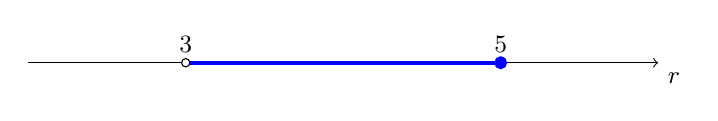
\begin{tikzpicture}[font=\small,x=10mm, y=5mm]

\draw[->] (0,0) -- (8,0) node [below right] () {$r$};
\node[above]  at (2,0) {$3$};
\node[above]  at (6,0) {5};
\begin{scope}[blue,ultra thick]
\draw (2,0) -- (6,0);
\draw[fill=blue] (6,0)circle (1.5pt);
\end{scope}
\draw[fill=white] (2,0)circle (1.5pt);

\end{tikzpicture}

  \boxA\quad~$x<5;x>3$\quad\boxB\quad~$3>x\ge~5$\quad\boxC\quad~$3\le x<5$\quad\boxD\quad~$3<x\le~5$
 \end{center}
  \end{esercizio}

\begin{esercizio}
 \label{ese:18.5}
Determina la scrittura corretta per il seguente grafico.
 \begin{center}
  % (c) 2012 Dimitrios Vrettos - d.vrettos@gmail.com
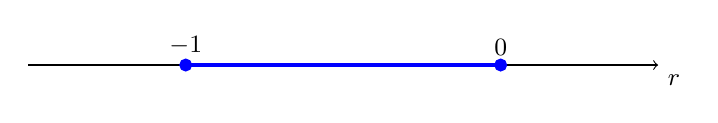
\begin{tikzpicture}[font=\small,x=10mm, y=5mm]

\draw[->] (0,0) -- (8,0) node [below right] () {$r$};
\node[above]  at (2,0) {$-1$};
\node[above]  at (6,0) {0};
\begin{scope}[blue,ultra thick]
\draw (2,0) -- (6,0);
\draw[fill=blue] (2,0)circle (1.5pt);
\draw[fill=blue] (6,0)circle (1.5pt);
\end{scope}

\end{tikzpicture}

  \boxA\quad~$\insR^{-}-\{-1\}$\quad\boxB\quad~$-1\ge x\ge~0$\quad\boxC\quad~$-1\le x\le~0$\quad\boxD\quad~$0<x<-1$
 \end{center}
 \end{esercizio}

\begin{esercizio}
 \label{ese:18.6}
Determina la scrittura corretta per il seguente grafico.
 \begin{center}
  % (c) 2012 Dimitrios Vrettos - d.vrettos@gmail.com
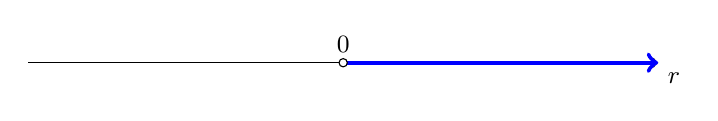
\begin{tikzpicture}[font=\small,x=10mm, y=5mm]

\draw[->] (0,0) -- (8,0) node [below right] () {$r$};
\node[above]  at (4,0) {0};
\begin{scope}[blue,ultra thick,->]
\draw (4,0) -- (8,0);
\end{scope}
\draw[fill=white] (4,0)circle (1.5pt);

\end{tikzpicture}

  \boxA\quad~$x>0$\quad\boxB\quad~$x>-\infty $\quad\boxC\quad~$x\le~0$\quad\boxD\quad~$0<x\le~0$
 \end{center}
  \end{esercizio}

\begin{esercizio}
 \label{ese:18.7}
Determina la scrittura corretta per il seguente grafico.
 \begin{center}
  % (c) 2012 Dimitrios Vrettos - d.vrettos@gmail.com
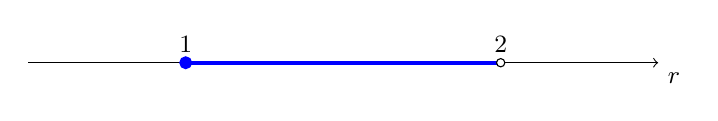
\begin{tikzpicture}[font=\small,x=10mm, y=5mm]

\draw[->] (0,0) -- (8,0) node [below right] () {$r$};
\node[above]  at (2,0) {$1$};
\node[above]  at (6,0) {2};
\begin{scope}[blue,ultra thick]
\draw (2,0) -- (6,0);
\draw[fill=blue] (2,0)circle (1.5pt);
\end{scope}
\draw[fill=white] (6,0)circle (1.5pt);

\end{tikzpicture}

  \boxA\quad~$x\ge~1;x<2$\quad\boxB\quad~$1\le x<2$\quad\boxC\quad~$x\le~1\text{ e }x>2$\quad\boxD\quad~$2\ge~1$
 \end{center}
  \end{esercizio}

\subsubsection*{18.2 - Disequazioni numeriche}
\begin{esercizio}
 \label{ese:18.8}
Completa la seguente tabella indicando con una crocetta il tipo di
disuguaglianza o disequazione:

 \begin{tabularx}{.9\textwidth}{Xccc}
 \toprule
 Proposizione&\multicolumn{2}{c}{Disuguaglianza}& Disequazione\\
  & Vera & Falsa & \\
 \midrule
 Il doppio di un numero reale è minore del suo triplo aumentato di~1: & & & \\
 La somma del quadrato di~4 con~3 è maggiore della somma del quadrato di~3 con~4: & & &\\
 Il quadrato della somma di~4 con~3 è minore o uguale a~49: & & & \\
 In~$\insZ:(5+8)-(2)^{4}>0$: & & & \\
 $-x^{2}>0$: & & & \\
 $(x+6)^{2}\cdot (1-9)\cdot (x+3-9)<0$: & & & \\
 \bottomrule
 \end{tabularx}
\end{esercizio}

\begin{esercizio}
 \label{ese:18.9}
 Rappresenta graficamente l'insieme delle soluzioni
delle seguenti disequazioni.
\begin{multicols}{3}
 \begin{enumeratea}
 \item $x-2>0$;
\item $x+5>0$;
\item $x-4>0$;
\item $x-5\ge~0$;
\item $x+3\le~0$;
\item $x>0$;
\item $x\ge~0$;
\item $-1\le x$;
\item $3>x$.
 \end{enumeratea}
\end{multicols}
\end{esercizio}

\begin{esercizio}[\Ast]
 \label{ese:18.10}
Trova l'Insieme Soluzione delle seguenti disequazioni.
\begin{multicols}{2}
 \begin{enumeratea}
 \item $3-x>x$;
\item $2x>3$;
\item $3x\le~4$;
\item $5x\ge -4$;
\item $x^{2}+x^{4}+10>0$;
\item $x^{2}+x^{4}+100<0$;
\item $-x+3>0$;
\item $-x-3\le~0$.
\end{enumeratea}
\end{multicols}
\end{esercizio}

\begin{esercizio}[\Ast]
 \label{ese:18.11}
Trova l'Insieme Soluzione delle seguenti disequazioni.
 \begin{multicols}{2}
 \begin{enumeratea}
 \item $3+2x\ge~3x+2$;
\item $5x-4\ge~6x-4$;
\item $-3x+2\ge -x-8$;
\item $4x+4\ge~2(2x+8)$;
\item $4x+4\ge~2(2x+1)$;
\item $4x+4\ge~2(2x+2)$;
\item $4x+4<2(2x+3)$;
\item $4x+4>2(2x+2)$.
\end{enumeratea}
\end{multicols}
\end{esercizio}

\begin{esercizio}[\Ast]
 \label{ese:18.12}
Trova l'Insieme Soluzione delle seguenti disequazioni.
 \begin{multicols}{2}
 \begin{enumeratea}
 \item $4x+4<2(2x+2)$;
\item $x^{2}+4>3$;
\item $x^{2}+3<-1$;
\item $-3x-8\ge~2$;
\item $-3x>0$;
\item $-3x\le~0$;
\item $-3x+5\ge~0$;
\item $-3x-8\ge~0$.
\end{enumeratea}
\end{multicols}
\end{esercizio}

\pagebreak

\begin{esercizio}[\Ast]
 \label{ese:18.13}
Trova l'Insieme Soluzione delle seguenti disequazioni.
 \begin{multicols}{2}
 \begin{enumeratea}
 \item $4x+4\ge~3\left(x+\frac{4}{3}\right)$;
\item $-{\dfrac{4}{3}}x\ge~1$;
\item $-{\dfrac{4}{3}}x\ge~0$;
\item $-{\dfrac{4}{3}}x\ge \dfrac{2}{3}$;
\item $-{\dfrac{2}{3}}x\le \dfrac{1}{9}$;
\item $-{\dfrac{2}{3}}x\le~9$;
\item $\dfrac{x+5}{2}>-{\dfrac{1}{5}}$;
\item $x^2+1\ge\dfrac{x^2+4x-1}{2}+3x$.
\end{enumeratea}
\end{multicols}
\end{esercizio}

\begin{esercizio}[\Ast]
 \label{ese:18.14}
Trova l'Insieme Soluzione delle seguenti disequazioni.
 \begin{multicols}{2}
 \begin{enumeratea}
 \item $x+\dfrac{1}{2}<\dfrac{(x+3)}{3}-1$;
\item $\dfrac{(x+5)}{3}+3+2\dfrac{(x-1)}{3}\le x+4$;
\item $(x+3)^{2}\ge (x-2)(x+2)$;
\item $\dfrac{3}{2}x+\dfrac{1}{4}<5\left(\dfrac{2}{3}x-\dfrac{1}{2}\right)$;
\item $1-(2x-4)^{2}>-x\cdot (4x+1)+2$;
\item $(x+1)^{2}\ge (x-1)^{2}$;
\item $\dfrac{3}{2}\cdot (x+1)-\dfrac{1}{3}\cdot (1-x)<x+2$;
\item $\dfrac{x+\np{0,25}}{2}<\np{1,75}+\np{0,25}x$.
\end{enumeratea}
\end{multicols}
\end{esercizio}

\begin{esercizio}[\Ast]
 \label{ese:18.15}
Trova l'Insieme Soluzione delle seguenti disequazioni.
 \begin{multicols}{2}
 \begin{enumeratea}
\item $x-3(x+3)<x-2(x-1)$;
\item $2(1+2x)>1-2x$;
\item $1+x^{2}<-5+(x-1)^{2}+x+1$;
\item $(x-3)^{2}+1+4x+3(x-1)>(x+2)^{2}$;
\item $\dfrac{-2+3x}{3}<\dfrac{x-1}{4}+\dfrac{x-2}{6}$;
\item $\dfrac{x-1}{5}-\dfrac{4x-1}{10}>\dfrac{1-x}{2}$.
\end{enumeratea}
\end{multicols}
\end{esercizio}

\begin{esercizio}[\Ast]
 \label{ese:18.16}
Trova l'Insieme Soluzione delle seguenti disequazioni.
 \begin{multicols}{2}
 \begin{enumeratea}
\item $3x+1+\dfrac{x}{6}+\dfrac{1}{3}\left(2-\dfrac{x+5}{2}\right)>\dfrac{x+8}{6}$;
\item $\dfrac{(x+1)^{2}}{8}+\dfrac{2+x}{2}<1+x+2\left(\dfrac{x-1}{4}\right)^{2}$;
\item $x-1-4<\dfrac{4+x}{8}+\dfrac{3(3x-1)}{4}+\dfrac{2x-1}{2}$;
\item $\dfrac{x-1}{2}+\dfrac{3x+1}{2}>2x$;
\item $\dfrac{2x-3}{3}>\dfrac{x-2}{2}+\dfrac{3x-5}{6}$;
\item $\dfrac{2(5x+1)}{3}-4>\dfrac{x-1}{2}$.
\end{enumeratea}
\end{multicols}
\end{esercizio}

\begin{esercizio}[\Ast]
 \label{ese:18.17}
Trova l'Insieme Soluzione delle seguenti disequazioni.
 \begin{enumeratea}
 \item $\dfrac{1}{2}\left(3x-\dfrac{1}{3}\right)+\dfrac{1}{3}(1+x)(1-x)+3\left(\dfrac{1}{3}x-1\right)^{2}\ge~0$;
\item $3\dfrac{(x+1)}{2}-\dfrac{x+1}{3}-\dfrac{1}{9}>-5x+\dfrac{1}{2}$;
\item $\left(\dfrac{x}{2}-1\right)\left(1+\dfrac{x}{2}\right)+x-\dfrac{1}{2}>x\dfrac{(x-1)}{4}+\dfrac{5x-6}{4}$;
\item $\dfrac{1}{2}\left(x-\dfrac{1}{2}\right)+\dfrac{1}{3}\left(x+\dfrac{1}{3}\right)>\dfrac{x-\dfrac{1}{2}}{3}+\dfrac{x-\dfrac{1}{3}}{2}$.
\end{enumeratea}
\end{esercizio}
\begin{multicols}{2}
\begin{esercizio}[\Ast]
 \label{ese:18.18}
 Sommando un numero con il doppio del suo successivo si deve ottenere
un numero maggiore di~17. Quali numeri verificano questa
condizione?
\end{esercizio}

 \begin{esercizio}[\Ast]
 \label{ese:18.19}
 Sommando due numeri pari consecutivi si deve ottenere un numero che
non supera la metà del numero più grande. Quali valori può
assumere il primo numero pari?
 \end{esercizio}

 \begin{esercizio}[\Ast]
 \label{ese:18.20}
 Il noleggio di una automobile costa \officialeuro~$\np{55,00}$ al giorno, più
\officialeuro~$\np{0,085}$ per ogni chilometro percorso. Qual è il massimo di
chilometri da percorrere giornalmente, per spendere non più di \officialeuro~$\np{80,00}$ al giorno?
 \end{esercizio}

 \begin{esercizio}
 \label{ese:18.21}
 In una fabbrica, per produrre una certa merce, si ha
una spesa fissa settimanale di \officialeuro~$413$, ed un costo di produzione di \officialeuro~$\np{2,00}$ per ogni
kg di merce. Sapendo che la merce viene venduta a \officialeuro~$\np{4,00}$ al~kg, determinare la quantità minima da produrre
alla settimana perché l'impresa non sia in perdita.
 \end{esercizio}

 \begin{esercizio}[\Ast]
 \label{ese:18.22}
 Per telefonare in alcuni paesi esteri, una compagnia telefonica
propone due alternative di contratto:
\begin{enumeratea}
 \item \officialeuro~$\np{1,20}$ per il primo minuto di conversazione, \officialeuro~$\np{0,90}$ per ogni minuto successivo;
\item \officialeuro~$\np{1,00}$ per ogni minuto di conversazione.
\end{enumeratea}
Quanti minuti deve durare una telefonata perché convenga la seconda
alternativa?
 \end{esercizio}

\begin{esercizio}[\Ast]
 \label{ese:18.23}
 Il prezzo di un abbonamento mensile ferroviario è di \officialeuro~$\np{125,00}$.
 Sapendo che il prezzo di un singolo biglietto sulla stessa
tratta è di \officialeuro~$\np{9,50}$, trovare il numero minimo di viaggi per
cui l'abbonamento mensile risulta conveniente, e
rappresentare graficamente la soluzione.
 \end{esercizio}

 \begin{esercizio}
 \label{ese:18.24}
 Al circolo di tennis i soci pagano \officialeuro~$12$ a ora di gioco, mentre i non
soci pagano \officialeuro~$15$. Sapendo che la tessera annuale costa
\officialeuro~$150$, qual è il numero minimo di partite all'anno oltre il quale risulta conveniente
fare la tessera di socio?
 \end{esercizio}

 \begin{esercizio}[\Ast]
 \label{ese:18.25}
 \ In montagna l'abbonamento per due settimane allo
skipass costa \officialeuro~$220$ mentre il biglietto giornaliero costa
\officialeuro~$20$. Andando a sciare ogni giorno, dopo quanti giorni risulta coneniente
fare l'abbonamento?
 \end{esercizio}

 \begin{esercizio}[\Ast]
 \label{ese:18.26}
 Marco ha preso alle prime tre prove di matematica i seguenti voti: $5$;
$\np{5,5}$; $\np{4,5}$. Quanto deve prendere alla quarta e ultima prova per avere almeno~$6$
di media?
 \end{esercizio}

 \begin{esercizio}
 \label{ese:18.27}
 Per produrre un tipo di frullatore, un'azienda ha dei
costi fissi per \officialeuro~$\np{12000}$ a settimana e riesce a produrre~$850$
frullatori a settimana, ognuno dei quali ha un costo di produzione pari
a \officialeuro~$34$. L'azienda concorrente riesce a
vendere un frullatore analogo a \officialeuro~$79$. A quanto devono essere
venduti i frullatori in modo che l'azienda abbia un
utile e che il prezzo di vendita non sia superiore a quello del
prodotto concorrente?
 \end{esercizio}

 \begin{esercizio}[\Ast]
 \label{ese:18.28}
 Per il noleggio, una compagnia propone
un'auto di tipo citycar al costo di \officialeuro~$\np{0,20}$ per km percorso e una quota fissa giornaliera
di \officialeuro~$\np{15,00}$,
un'auto di tipo economy al costo di \officialeuro~$\np{0,15}$
per km e una quota fissa giornaliera di \officialeuro~$\np{20,00}$. Dovendo
noleggiare l'auto per~3 giorni, quanti km occorre fare
perché sia più conveniente l'auto di tipo economy?
 \end{esercizio}

 \begin{esercizio}
 \label{ese:18.29}
 Alle~9:00 di mattina sono in autostrada e devo raggiungere una città
che dista~$740\unit{km}$ entro le~17:00 poiché ho un appuntamento di lavoro.
Prevedendo una sosta di mezz'ora per mangiare un panino, a quale
velocità devo viaggiare per arrivare in orario?
 \end{esercizio}

 \begin{esercizio}[\Ast]
 \label{ese:18.30}
 Quanto deve essere lungo il lato di un triangolo equilatero il cui
perimetro deve superare di~$900\unit{cm}$ il perimetro di un triangolo
equilatero che ha il lato di~$10\unit{cm}$?
 \end{esercizio}

 \begin{esercizio}[\Ast]
 \label{ese:18.31}
 I lati di un triangolo sono tali che il secondo è doppio del primo e
il terzo è più lungo del secondo di~$3\unit{cm}$. Se il perimetro deve
essere compreso tra~$10\unit{cm}$ e~$20\unit{cm}$, tra quali valori può variare il lato
più piccolo?
 \end{esercizio}

 \begin{esercizio}[\Ast]
 \label{ese:18.32}
 In un triangolo isoscele l'angolo
alla base deve essere minore della metà dell'angolo
al vertice. Tra quali valori deve essere compresa la misura
dell'angolo alla base?
 \end{esercizio}

 \begin{esercizio}[\Ast]
 \label{ese:18.33}
 Un trapezio rettangolo ha l'altezza che è il triplo
della base minore, mentre la sua base maggiore è~5 volte quella minore.
Se il perimetro del trapezio non deve superare i~$100\unit{m}$, quali valori
può assumere la lunghezza dell'altezza del
trapezio?
 \end{esercizio}

 \begin{esercizio}[\Ast]
 \label{ese:18.34}
 Un rettangolo ha la lunghezza dei lati una doppia dell'altra.
Si sa che il perimetro non deve superare~$600\unit{m}$ e che
l'area non deve essere inferiore a~$200\unit{m^2}$. Tra quali
valori possono variare le dimensioni del rettangolo?
 \end{esercizio}
\end{multicols}

 \subsubsection*{18.3 - Sistemi di disequazioni}

\begin{esercizio}
 \label{ese:18.35}
Sulla retta reale rappresenta l'insieme soluzione~$S_{1}$
dell'equazione:
\[\frac{1}{6}+\frac{1}{4}\cdot (5x+3)=2+\frac{2}{3}\cdot (x+1)\]
%\newpage
e l'insieme soluzione~$S_{2}$ della disequazione:
\[\frac{1}{2}-2\cdot\left(\frac{1-x}{4}\right)\ge~3-\frac{6-2x}{3}-\frac{x}{2}.\]

È vero che~$S_{1}\subset S_{2}$?
\end{esercizio}

\begin{esercizio}[\Ast]
 \label{ese:18.36}
 Determina i numeri reali che verificano il sistema:
 $\left\{%
  \begin{array}{l}
  x^{2}\le~0
  \\2-3x\ge~0
 \end{array}\right..$
 \end{esercizio}

\begin{esercizio}
 \label{ese:18.37}
 Attribuire il valore di verità alle seguenti proposizioni:

\begin{enumeratea}
\item il quadrato di un numero reale è sempre positivo;
\item l'insieme complementare di~$A=\{x\in\insR\;|\;x>-8\}\text{ è }B=\{x\in\insR \mid x<-8\}$;
\item il monomio~$-6x^{3}y^{2}$ assume valore positivo per tutte le coppie dell'insieme~$\insR^{+}\times\insR^{+}$;
\item nell'insieme~$\insZ$ degli interi relativi il sistema~$\left\{\begin{array}{l}x+1>0\\8x<0\end{array}\right.$ non ha soluzione;
\item l'intervallo~$\left[-1\text{,~}\left.-{\dfrac{1}{2}}\right)\right.$ rappresenta l'$\IS$ del sistema~$\left\{\begin{array}{l}1+2x<0 \\\dfrac{x+3}{2}\le x+1\end{array}\right.$.
\end{enumeratea}
\end{esercizio}

\begin{esercizio}[\Ast]
 \label{ese:18.38}
 Risolvi i seguenti sistemi di disequazioni.
 \begin{multicols}{2}
 \begin{enumeratea}
 \item $\left\{\begin{array}{l}
	3-x>x\\
	2x>3
	\end{array}\right.;$
\item $\left\{\begin{array}{l}
	3x\le~4\\
	5x\ge -4
   \end{array}\right.;$
\item $\left\{\begin{array}{l}
	2x>3\\
	3x\le~4
	\end{array}\right.;$
\item $\left\{\begin{array}{l}
	3x-5<2\\
	x+7<-2x
   \end{array}\right..$
 \end{enumeratea}
\end{multicols}
\end{esercizio}

\begin{esercizio}[\Ast]
 \label{ese:18.39}
 Risolvi i seguenti sistemi di disequazioni.
 \begin{multicols}{2}
 \begin{enumeratea}
 \item $\left\{\begin{array}{l}
	3-x\ge x-3\\
	-x+3\ge~0
	\end{array}\right.;$
\item $\left\{\begin{array}{l}
	-x-3\le~3\\
	3+2x\ge~3x+2
   \end{array}\right.;$
\item $\left\{\begin{array}{l}
	2x-1>2x \\
	3x+3\le~3
	\end{array}\right.;$
\item $\left\{\begin{array}{l}
	2x+2<2x+3\\
	2(x+3)>2x+5
	\end{array}\right..$
\end{enumeratea}
\end{multicols}
\end{esercizio}

\begin{esercizio}[\Ast]
 \label{ese:18.40}
 Risolvi i seguenti sistemi di disequazioni.
 \begin{multicols}{2}
 \begin{enumeratea}
 \item $\left\{\begin{array}{l}
	-3x>0\\
	-3x+5\ge~0\\
	-3x\ge-2x
	\end{array}\right.;$
\item {\longarray $\left\{\begin{array}{l}
	-{\dfrac{4}{3}}x\ge\dfrac{2}{3}\\
	-{\dfrac{2}{3}}x\le\dfrac{1}{9}
	\end{array}\right.;$}
\item $\left\{\begin{array}{l}
	3+2x>3x+2 \\
	5x-4\le~6x-4\\
	-3x+2\ge -x-8
	\end{array}\right.;$
\item $\left\{\begin{array}{l}
	4x+4\ge~3\cdot\left(x+\dfrac{4}{3}\right)\\
	4x+4\ge~2\cdot (2x+2)
	\end{array}\right..$
\end{enumeratea}
\end{multicols}
\end{esercizio}

\begin{esercizio}[\Ast]
 \label{ese:18.41}
 Risolvi i seguenti sistemi di disequazioni.
 \begin{multicols}{2}
 \begin{enumeratea}
 \item $\left\{\begin{array}{l}
	3(x-1)<2(x+1)\\
	x-\dfrac{1}{2}+\dfrac{x+1}{2}>0
	\end{array}\right.;$
\item {\longarray $\left\{\begin{array}{l}
	16(x+1)-2+(x-3)^{2}\le(x+5)^{2}\\
	\dfrac{x+5}{3}+3+2\cdot\dfrac{x-1}{3}\le x+4
	\end{array}\right.;$}
\item {\longarray $\left\{\begin{array}{l}
	x+\dfrac{1}{2}<\dfrac{1}{3}(x+3)-1\\
	(x+3)^{2}\ge (x-2)(x+2)
	\end{array}\right.;$}
\item {\longarray $\left\{\begin{array}{l}
	\dfrac{2x+3}{3}>x-1\\
	\dfrac{x-4}{5}<\dfrac{2x+1}{3}
	\end{array}\right..$}
\end{enumeratea}
\end{multicols}
\end{esercizio}

\begin{esercizio}[\Ast]
 \label{ese:18.42}
 Risolvi i seguenti sistemi di disequazioni.
 \begin{multicols}{2}
 \begin{enumeratea}
 \item $\left\{\begin{array}{l}
	(x-1)^{2}>1+(x+1)^{2}\\
	x^{2}+1<x(x+2)-x
	\end{array}\right.;$
\item {\longarray $\left\{\begin{array}{l}
	x+2>\dfrac{2}{3}(x-1)\\
	\dfrac{1}{2}-\dfrac{x-1}{4}>\dfrac{x+2}{5}-\dfrac{x+2}{3}
	\end{array}\right.;$}
\item {\longarray $\left\{\begin{array}{l}
	\dfrac{x-1}{4}<x\\
	\dfrac{x-1}{3}>\dfrac{x+1}{2}
	\end{array}\right.;$}
\item {\longarray $\left\{\begin{array}{l}
	\dfrac{16+5x}{5}>\dfrac{x+1}{5}+3\left(1-\dfrac{x}{2}\right)\\
	\dfrac{x-1}{9}+\dfrac{x+4}{3}>\dfrac{37}{18}+\dfrac{x-5}{6}
	\end{array}\right..$}
\end{enumeratea}
\end{multicols}
\end{esercizio}

\begin{esercizio}[\Ast]
 \label{ese:18.43}
 Risolvi i seguenti sistemi di disequazioni.
 \begin{multicols}{2}
 \begin{enumeratea}
\item {\longarray $\left\{\begin{array}{l}
	\dfrac{x-2}{6}>\dfrac{x-1}{2}+\dfrac{2x+1}{3}\\
	\dfrac{x+1}{4}<\dfrac{2-x}{3}-\dfrac{x-1}{6}\\
	\dfrac{x-5}{4}<-\dfrac{x-4}{5}+\dfrac{1}{20}x
	\end{array}\right.;$}
\item {\longarray $\left\{\begin{array}{l}
	\dfrac{x-7}{4}>\dfrac{2}{3}(x-1)-\dfrac{7(x+1)}{12}\\ %+\dfrac{x+3}{4}\\
	\dfrac{x-7}{8}+\dfrac{x+1}{6}>3x-15+\dfrac{x-2}{4}\\
	3>\dfrac{x+4}{2}+\dfrac{1-2x}{3}
	\end{array}\right.;$}
\item $\left\{\begin{array}{l}
	9<-x\\
	3-x>-1-4(x+1)\\
	3x-1<7-2x
	\end{array}\right.;$
\item {\longarray $\left\{\begin{array}{l}
	\dfrac{3}{7}x-2<\dfrac{5x-7}{14}-\dfrac{2x+7}{21}\\
	2x-5-\dfrac{2x-11}{2}>\dfrac{19-2x}{2}-\dfrac{5}{2}x\\
	\dfrac{13}{2}-2x+\dfrac{9-3x}{10}<\dfrac{5x-12}{6}\\
	\dfrac{7}{2}-x-\dfrac{1}{3}x<\dfrac{4x-1}{4}-\dfrac{x+9}{3}
	\end{array}\right..$}
\end{enumeratea}
\end{multicols}
\end{esercizio}

\pagebreak

\begin{esercizio}[\Ast]
 \label{ese:18.44}
 Risolvi i seguenti sistemi di disequazioni.

 \begin{enumeratea}
 \item {\longarray $\left\{\begin{array}{l}
	2\left(x-\dfrac{1}{3}\right)+x>3x-2\\
	\dfrac{x}{3}-\dfrac{1}{2}\ge \dfrac{x}{4}-\dfrac{x}{6}
   \end{array}\right.;$}
\item $\left\{\begin{array}{l}
    \dfrac{3}{2}x+\dfrac{1}{4}<5\cdot\left(\dfrac{2}{3}x-\dfrac{1}{2}\right)\\
    x^2-2x+1\ge~0
   \end{array}\right.;$
\item {\longarray $\left\{\begin{array}{l}
	3\left(x-\dfrac{4}{3}\right)+\dfrac{2-x}{3}+x-\dfrac{x-1}{3}>0\\
	\left[1-\dfrac{1}{6}(2x+1)\right]+\left(x-\dfrac{1}{2}\right)^{2}<(x+1)^{2}+\dfrac{1}{3}(1+2x)
   \end{array}\right.;$}
\item {\longarray $\left\{\begin{array}{l}
	\left(x-\dfrac{1}{2}\right)\left(x+\dfrac{1}{2}\right)>\left(x-\dfrac{1}{2}\right)^{2}\\
	2\left(x-\dfrac{1}{2}\right)\left(x+\dfrac{1}{2}\right)<\left(x-\dfrac{1}{2}\right)^{2}+\left(x+\dfrac{1}{2}\right)^{2}
   \end{array}\right.;$}
\item {\longarray $\left\{\begin{array}{l}
  (x+3)^{3}-(x+3)(9x-2)>x^{3}+27\\
  \dfrac{x+5}{3}+3+\dfrac{2(x-1)}{3}<x+1
 \end{array}\right..$}
 \end{enumeratea}
\end{esercizio}

\subsubsection*{18.4 - Disequazioni polinomiali di grado superiore al primo}
\begin{esercizio}
 \label{ese:18.45}
 Mediante il metodo~1 del problema~\ref{pro:18.1} (a pagina \pageref{pro:18.1}) risolvi le seguenti disequazioni.

\begin{enumeratea}
\item $(x+3)\cdot \left(\frac{1}{5}x+\frac{3}{2}\right)<0$ e~$\left(-{\frac{6}{11}}+2x\right)\cdot\left(-x+\frac{9}{2}\right)$;
\item $\left(x+\frac{3}{2}\right)\cdot \left(5x+\frac{1}{5}\right)<0$ e~$\left(-{\frac{1}{10}}x+2\right)\cdot \left(-3x+9\right)\ge~0$.
\end{enumeratea}

\end{esercizio}

\begin{esercizio}
 \label{ese:18.46}
 Il metodo~1 del problema~\ref{pro:18.1} (a pagina \pageref{pro:18.1}) si complica se il prodotto ha
più di due fattori. Prova infatti ad applicarlo alla seguente
disequazione:
$(x-3)\cdot (2x-9)\cdot (4-5x)>0.$
\end{esercizio}

\begin{esercizio}[\Ast]
 \label{ese:18.47}
Trova l'Insieme Soluzione delle seguenti disequazioni.
\begin{multicols}{2}
 \begin{enumeratea}
 \item $(x+2)(3-x)\le~0$;
\item $x(x-2)>0$;
\item $(3x+2)(2-3x)<0$;
\item $-3x(2-x)(3-x)\ge~0$.
\end{enumeratea}
\end{multicols}
\end{esercizio}

\begin{esercizio}[\Ast]
 \label{ese:18.48}
Trova l'Insieme Soluzione delle seguenti disequazioni.
\begin{multicols}{2}
 \begin{enumeratea}
 \item $(x+1)(1-x)\left(\frac{1}{2}x-2\right)\ge~0$;
\item $(x-1)(x-2)(x-3)(x-4)<0$;
\item $x^{2}-16\le~0$;
\item $4x^{2}-2x<0$.
\end{enumeratea}
\end{multicols}
\end{esercizio}

\begin{esercizio}[\Ast]
 \label{ese:18.49}
Trova l'Insieme Soluzione delle seguenti disequazioni.
\begin{multicols}{2}
 \begin{enumeratea}
 \item $x^{4}-81\ge~0$;
\item $x^{2}+17x+16\le~0$;
\item $16-x^{4}\le~0$;
\item $x^{2}+2x+1<0$.
\end{enumeratea}
\end{multicols}
\end{esercizio}

\pagebreak

\begin{esercizio}[\Ast]
 \label{ese:18.50}
Trova l'Insieme Soluzione delle seguenti disequazioni.
\begin{multicols}{2}
 \begin{enumeratea}
 \item $x^{2}+6x+9\ge~0$;
\item $x^{2}-5x+6<0$;
\item $x^{2}+3x-4\le~0$;
\item $x^{3}>x^{2}$.
\end{enumeratea}
\end{multicols}
\end{esercizio}

\begin{esercizio}[\Ast]
 \label{ese:18.51}
Trova l'Insieme Soluzione delle seguenti disequazioni.
\begin{multicols}{2}
 \begin{enumeratea}
 \item $x^{2}(2x^{2}-x)-(2x^{2}-x)<0$;
\item $x^{2}-2x+1+x(x^{2}-2x+1)<0$;
\item $x^{3}-2x^{2}-x+2\ge~0$;
\item $x^{4}+4x^{3}+3x^{2}>0$.
\end{enumeratea}
\end{multicols}
\end{esercizio}

\begin{esercizio}[\Ast]
 \label{ese:18.52}
Trova l'Insieme Soluzione delle seguenti disequazioni.
\begin{multicols}{2}
 \begin{enumeratea}
 \item $(6x^{2}-24x)(x^{2}-6x+9)<0$;
\item $(x^{3}-8)(x+2)<(2-x)(x^{3}+8)$;
\item $(2a+1)(a^{4}-2a^{2}+1)<0$;
\item $x^{3}-6x^{2}+11>1-3x$;
\item $x^{6}-x^{2}+x^{5}-6x^{4}-x+6<0$.
\end{enumeratea}
\end{multicols}
\end{esercizio}

\begin{esercizio}[\Ast]
 \label{ese:18.53}
 Determina i valori che attribuiti alla variabile~$y$ rendono positivi
entrambi i polinomi
seguenti:~$p_{1}=y^{4}-13y^{2}+36;\quad p_{2}=y^{3}-y^{2}-4y+4.$
\end{esercizio}

\begin{esercizio}[\Ast]
 \label{ese:18.54}
 Determina i valori di~$a$ che rendono~$p=a^{2}+1$ minore di~5.
\end{esercizio}

\begin{esercizio}[\Ast]
 \label{ese:18.55}
 Determina~$\IS$ dei seguenti sistemi di disequazioni.
 \begin{multicols}{3}
 \begin{enumeratea}
 \item $\left\{\begin{array}{l}
		x^{2}-9\ge~0\\
		x^{2}-7x+10<0
	   \end{array}\right.;$
\item $\left\{\begin{array}{l}
		x^{2}+3x-18\ge~0\\
		12x^{2}+12x+3>0
	   \end{array}\right.;$
\item $\left\{\begin{array}{l}
		16x^{4}-1<0 \\
		16x^{3}+8x^{2}\ge~0 \end{array}\right.. $
 \end{enumeratea}
 \end{multicols}
\end{esercizio}

\begin{esercizio}[\Ast]
 \label{ese:18.56}
 Determina~$\IS$ dei seguenti sistemi di disequazioni.
 \begin{multicols}{2}
 \begin{enumeratea}
 \item $\left\{\begin{array}{l}
		49a^{2}-1\ge~0\\
		9a^{2}<1\\
		1-a>0
	   \end{array}\right.;$

\item $\left\{\begin{array}{l}
	  2x^{2}-13x+6<0\\
	  (2x^{2}-5x-3)(1-3x)>0\\
	  x^{2}+7>1
	   \end{array}\right..$
 \end{enumeratea}
 \end{multicols}
\end{esercizio}

\subsubsection*{18.5 - Disequazioni frazionarie}

\begin{esercizio}
\label{ese:18.57}
Studia il segno della frazione
\[f=\dfrac{x^{3}+11x^{2}+35x+25}{x^{2}-25}.\]
\emph{Traccia di svolgimento}. Scomponi in fattori numeratore e denominatore, otterrai
\[ f=\frac{(x+5)^{2}(x+1)}{(x+5)(x-5)}.\]
Poni le~$\CE$ e semplifica la frazione: \dotfill

Studia separatamente il segno di tutti i fattori che vi compaiono. Verifica che la tabella dei segni sia:
\begin{center}
% (c) 2012 Dimitrios Vrettos - d.vrettos@gmail.com
\begin{tikzpicture}[font=\small,x=10mm, y=10mm]

\draw[->] (0,0) -- (8,0) node [below right] () {$r$};

\foreach \x in {1.5,3.5,6.5}{
\draw(\x,3pt)--(\x,-3pt);
\begin{scope}[dotted]
\draw (\x,0) -- (\x,-2);
\draw (0,-.5) -- (1.5,-.5);
\draw (0,-1) -- (3.5,-1);
\draw (0,-1.5) -- (6.5,-1.5);
\end{scope}}


\node[above] at (1.5,0) {$-5$};
\node[above]  at (3.5,0) {$-1$};
\node[above]  at (6.5,0) {$5$};

\begin{scope}[blue,thick]
\draw (1.5,-.5) -- (8,-.5);
\draw (3.5,-1) -- (8,-1);
\draw (6.5,-1.5) -- (8,-1.5);

\draw[fill=white] (1.5,-.5)circle (1.5pt);
\draw[fill=blue] (3.5,-1)circle (1.5pt);
\draw[fill=white] (6.5,-1.5)circle (1.5pt);
\end{scope}

\foreach \x in {-1.5}{
\node (n1) at (\x,-.25) {segno di $n_1$:};
\node(n2)  at (\x,-.75) {segno di $n_2$:};
\node   at (\x,-1.25) {segno di $D$:};
\node (d3) at (\x,-1.75) {segno di $f$:};
}

 \draw[decorate, decoration={brace, mirror}]  let \p1=(n1.north west), \p2=(n2.south west) in(\p1 ) -- (\p2) node[midway, left=2pt] {$N:$};

\foreach \z in {2.5,5,7.25}
\node  at (\z,-.25) {$+$};

 \foreach \zi in {.75,2.5}
 \node  at (\zi,-.75) {$-$};

\foreach \zii in {5,7.25}
 \node  at (\zii,-.75) {$+$};

 \foreach \ziii in {.75,2.5,5}
\node  at (\ziii,-1.25) {$-$};

\node  at (.75,-.25) {$-$};
\node  at (7.25,-1.25) {$+$};

\begin{scope}[red]
\foreach \y in {-1.75}{
\foreach \ziv in {.75,5}
	\node at (\ziv,\y) {$-$};
\foreach \zv in {2.5,7.25}
\node at (\zv,\y) {$+$};
}
\end{scope}
\end{tikzpicture}
\end{center}
La frazione assegnata, con la~$\CE: x\neq -5\text{ e }x\neq~5$, si annulla se~$x=-1$;
è positiva nell'insieme~$A^{+}=\left\{x\in \insR | -5<x<-1\vee x>5\right\}$ ed è negativa in
$A^{-}=\left\{x\in\insR | x<-5\vee -1<x<5\right\}$.
\end{esercizio}

\begin{esercizio}[\Ast]
\label{ese:18.58}
Determina~$\IS$ delle seguenti disequazioni fratte.
\begin{multicols}{2}
\begin{enumeratea}
\spazielenx
\item $\dfrac{x-2}{3x-9}>0$;
\item $\dfrac{3x+12}{(x-4)(6-3x)}\geqslant~0$;
\item $\dfrac{x+2}{x-1}<2$;
\item $\dfrac{4-3x}{6-5x}\geqslant -3$.
\end{enumeratea}
\end{multicols}
\end{esercizio}

\begin{esercizio}[\Ast]
\label{ese:18.59}
Determina~$\IS$ delle seguenti disequazioni fratte.
\begin{multicols}{2}
\begin{enumeratea}
\spazielenx
 \item $\dfrac{x+8}{x-2}\ge~0$;
\item $\dfrac{3x+4}{x^{2}+1}\ge~2$;
\item $\dfrac{4}{x+4}+\dfrac{2}{x-3}\leqslant~0$;
\item $\dfrac{7}{x+3}-\dfrac{6}{x+9}\geqslant~0$.
\end{enumeratea}
\end{multicols}
\end{esercizio}

\begin{esercizio}[\Ast]
\label{ese:18.60}
Determina~$\IS$ delle seguenti disequazioni fratte.
\begin{multicols}{2}
\begin{enumeratea}
\spazielenx
\item $\dfrac{3}{2-x}\leqslant \dfrac{1}{x-4}$;
\item $\dfrac{2}{4x-16}<\dfrac{2-6x}{x^{2}-8x+16}$;
\item $\dfrac{x-3}{x^{2}-4x+4}-1<\dfrac{3x-3}{6-3x}$;
\item $\dfrac{2}{x-2}>\dfrac{2x-2}{(x-2)(x+3)}$.
\end{enumeratea}
\end{multicols}
\end{esercizio}

\begin{esercizio}[\Ast]
\label{ese:18.61}
Determina~$\IS$ delle seguenti disequazioni fratte.
\begin{multicols}{2}
\begin{enumeratea}
\spazielenx
 \item $\dfrac{5}{2x+6}\geqslant \dfrac{5x+4}{x^{2}+6x+9}$;
\item $\dfrac{x}{x+1}-\dfrac{1}{x^{3}+1}\le~0$;
\item $\dfrac{(x+3)(10x-5)}{x-2}<0$;
\item $\dfrac{4-3x}{x-2}<\dfrac{3x+1}{x-2}$.
\end{enumeratea}
\end{multicols}
\end{esercizio}

\begin{esercizio}[\Ast]
\label{ese:18.62}
Determina~$\IS$ delle seguenti disequazioni fratte.
\begin{multicols}{2}
\begin{enumeratea}
\spazielenx
 \item $\dfrac{5x-4}{3x-12}\ge \dfrac{x-4}{4-x}$;
\item $\dfrac{2-x}{5x-15}\le \dfrac{5x-1}{2x-6}$;
\item $\dfrac{(3x-12)(6-x)}{(24-8x)(36-18x)}\leqslant~0$;
\item $\dfrac{(x-2)(5-2x)}{(5x-15)(24-6x)}\geqslant~0$.
\end{enumeratea}
\end{multicols}
\end{esercizio}
\pagebreak
\begin{esercizio}[\Ast]
\label{ese:18.63}
Determina~$\IS$ delle seguenti disequazioni fratte.
\begin{multicols}{2}
\begin{enumeratea}
\spazielenx
\item $\dfrac{(x-2)(x+4)(x+1)}{(x-1)(3x-9)(10-2x)}\leqslant~0$;
\item $\dfrac{(5-x)(3x+6)(x+3)}{(4-2x)(x-6)x}\leqslant~0$;
\item $\dfrac{(x-5)(3x-6)(x-3)}{(4-2x)(x+6)x}\leqslant~0$;
\item $\dfrac{(x-3)(x+2)(15+5x)}{x^{2}-5x+4}\geqslant~0$.
\end{enumeratea}
\end{multicols}
\end{esercizio}

\begin{esercizio}[\Ast]
\label{ese:18.64}
Determina~$\IS$ delle seguenti disequazioni fratte.
\begin{multicols}{2}
\begin{enumeratea}
\spazielenx
\item $\dfrac{\left(x-4\right)^{2}(x+3)}{x^{2}+5x+6}\geqslant~0$;
\item $\dfrac{x}{1-x^{2}}>\dfrac{1}{2x+2}-\dfrac{2}{4x-4}$;
\item $\dfrac{3-x}{x-2}<\dfrac{x-1}{x+3}+\dfrac{2}{x^{2}+x-6}$;
\item $\dfrac{2}{x+2}-\dfrac{1}{x+1}\ge \dfrac{3}{2x+2}$.
\end{enumeratea}
\end{multicols}
\end{esercizio}

\begin{esercizio}[\Ast]
\label{ese:18.65}
Determina~$\IS$ delle seguenti disequazioni fratte.
\begin{multicols}{2}
\begin{enumeratea}
\spazielenx
 \item $\dfrac{3}{2x-1}\le \dfrac{2x^{2}}{2x^{2}-x}-\dfrac{x+1}{x}$;
\item $\dfrac{2x^{2}}{2x^{2}-x}>1$;
\item $\dfrac{2x}{2x-1}+\dfrac{x+2}{2x+1}>\dfrac{3}{2}$;
\item $\dfrac{x^{2}-5x+6}{x^{2}-7x+12}\le~1$.
\end{enumeratea}
\end{multicols}
\end{esercizio}

\begin{esercizio}[\Ast]
\label{ese:18.66}
Determina~$\IS$ delle seguenti disequazioni fratte.
\begin{multicols}{2}
\begin{enumeratea}
\spazielenx
 \item $\dfrac{\dfrac{2}{x+1}}{x^{2}-1}<0$;
\item $\dfrac{x}{x+1}-\dfrac{4-x}{x+2}\ge \dfrac{2x+1}{x^{2}+3x+2}$;
\item $\dfrac{3}{2x^{2}-4x-6}-\dfrac{x-2}{3x+3}<\dfrac{x-1}{2x-6}$;
\item $\dfrac{1}{2-2x}\cdot \left(\dfrac{x(x-2)}{x-1}-\dfrac{3}{3-3x}\right)>-1$.
\end{enumeratea}
\end{multicols}
\end{esercizio}

\begin{esercizio}[\Ast]
\label{ese:18.67}
Determina~$\IS$ delle seguenti disequazioni fratte.
\begin{multicols}{2}
\begin{enumeratea}
\spazielenx
 \item $\dfrac{x+1}{2}-2-\dfrac{x-1}{x}>0$;
\item $\dfrac{x+15}{3x-9}-\dfrac{4}{x-3}>0$;
\item $\dfrac{2x+3}{x-1}>\dfrac{3}{1-x}-2$;
\item $\dfrac{3x}{x-2}+\dfrac{4}{x+2}<\dfrac{8-3x^{2}}{4-x^{2}}$.
\end{enumeratea}
\end{multicols}
\end{esercizio}

\begin{esercizio}[\Ast]
\label{ese:18.68}
Determina~$\IS$ delle seguenti disequazioni fratte.
\begin{multicols}{2}
\begin{enumeratea}
\spazielenx
\item $\dfrac{3x-5}{x-2}+\dfrac{2x-3}{2x-4}<\dfrac{x-3}{3x-6}$;
\item $\dfrac{1}{x-2}>3-\dfrac{1-3x}{2-x}$;
\item $\dfrac{9x+4}{x+1}-6>0$;
\item $\dfrac{x+5}{x-1}<1$.
\end{enumeratea}
\end{multicols}
\end{esercizio}

\begin{esercizio}[\Ast]
\label{ese:18.69}
Determina~$\IS$ delle seguenti disequazioni fratte.

\begin{enumeratea}
 \item $-{\dfrac{2}{27-3x^{2}}}-\dfrac{x+1}{2x-6}+\dfrac{3-2x}{6x-18}<-{\dfrac{3}{x^{2}-9}}+4\dfrac{x-3}{18-2x^{2}}$;
\item $\dfrac{2}{x^{2}-3x+2}-\dfrac{x}{x-2}<\dfrac{x-1}{x-1}-\dfrac{1}{3x-x^{2}-2}+\dfrac{2-x}{4x-4}$;
\item $\dfrac{(x-2)(x+4)(x^{2}+5x+6)}{(x^{2}-9)(-4-7x^{2})(x^{2}-6x+8)(x^{2}+4)}<0$.
\end{enumeratea}
\end{esercizio}

\begin{esercizio}
\label{ese:18.70}
Dopo aver ridotto ai minimi termini la frazione
$f=\dfrac{3x^{4}-2x^{3}+3x^{2}-2x}{6x^{2}-x-7}$, completa

 \begin{enumeratea}
 \item $f>0$ per~$x<-1$ oppure \dotfill
 \item $f=0$ per \dotfill
 \item $f<0$ per \dotfill
 \end{enumeratea}
\end{esercizio}

\begin{esercizio}
\label{ese:18.71}
Determina il segno delle frazioni, dopo averle ridotte ai minimi termini.
\[f_{1}=\dfrac{1-a^{2}}{2+3a};\quad f_{2}=\dfrac{a^{3}-5a^{2}-3+7a}{9-6a+a^{2}};\quad f_{3}=\dfrac{11m-m^{2}+26a}{(39-3m)(m^{2}+4m+4)}.\]
\end{esercizio}

\begin{esercizio}[\Ast]
\label{ese:18.72}
Risolvi i seguenti sistemi con disequazioni fratte.
\begin{multicols}{2}
\begin{enumeratea}{\longarray
 \item $\left\{\begin{array}{l}
		\dfrac{2x}{x-1}\ge~2\\
		\dfrac{x}{x-3}<0
	\end{array}\right.;$
\item $\left\{\begin{array}{l}
        \dfrac{1}{x}-\dfrac{1}{5}>\dfrac{2}{x}+1\\
        \dfrac{3x-3}{2x}>1+\dfrac{2}{x}
       \end{array}\right.;$
\item $\left\{\begin{array}{l}
        \dfrac{1}{x}-1\ge~0\\
        \dfrac{5+2x}{3x-2}<\dfrac{1}{2}
	   \end{array}\right.;$
\item $\left\{\begin{array}{l}
	   \dfrac{x+1}{x-1}-1>0\\
	   \dfrac{1}{2}x-\dfrac{1}{x}\le~\dfrac{1+x}{2}
	   \end{array}\right..$}
\end{enumeratea}
\end{multicols}
\end{esercizio}

\begin{esercizio}[\Ast]
\label{ese:18.73}
Risolvi i seguenti sistemi con disequazioni fratte.
\begin{multicols}{2}
\begin{enumeratea}{\longarray
 \item $\left\{\begin{array}{l}
		\dfrac{2-x}{3x^{2}+x}\ge~0\\
		x^{2}-x-6\ge~0\\
		x^{2}-4\le~0
	\end{array}\right.;$
\item $\left\{\begin{array}{l}
        \dfrac{x^{2}-4x+4}{9-x^{2}}>0\\
        x^{2}-3x\le~0
       \end{array}\right.;$
\item $\left\{\begin{array}{l}
	   \dfrac{1}{x-2}+\dfrac{3}{x+2}<0\\
	   \dfrac{2-x}{5x-15}\le\dfrac{5x-1}{2x-6}
	   \end{array}\right.;$
\item $\left\{\begin{array}{l}
	   \dfrac{4}{8-4x}-\dfrac{6}{2x-4}<0\\
	   \dfrac{x}{x-2}-\dfrac{6}{x^{3}-8}>1
	   \end{array}\right..$}
\end{enumeratea}
\end{multicols}
\end{esercizio}

\begin{esercizio}[\Ast]
\label{ese:18.74}
Risolvi i seguenti sistemi con disequazioni fratte.
\begin{multicols}{2}
\begin{enumeratea}{\longarray
 \item $\left\{\begin{array}{l}
		\dfrac{2}{1-x}\ge~-\dfrac{1}{x+2}\\
		\dfrac{1}{x^{2}-x}-\dfrac{1}{x}\ge~\dfrac{2}{x-1}
	\end{array}\right.;$
\item $\left\{\begin{array}{l}
        (2x+1)(x-1)(3-x)\ge~0\\
        \left(\dfrac{1}{3}x^{2}-3\right)-x\left(\dfrac{1}{3}x^{2}-3\right)>0
       \end{array}\right.;$
\item $\left\{\begin{array}{l}
	   x^{2}-4>x\left(x^{2}-4\right)\\
	   \dfrac{x}{x-1}\ge~-2\\
	   (x-1)^{2}-(x-2)^{2}<0
	   \end{array}\right.;$
\item $\left\{\begin{array}{l}
	   \left(1+\dfrac{2}{x-2}\right)\left(1-\dfrac{2}{x-2}\right)<\dfrac{x-4}{2-x}\\
	   \left(\dfrac{2-x}{(x-3)^{2}}+\dfrac{2+x}{x^{2}-9}\right)\cdot{\dfrac{x^{3}-27}{2x}}>0
	   \end{array}\right..$}
\end{enumeratea}
\end{multicols}

\end{esercizio}

\begin{esercizio}[\Ast]
\label{ese:18.75}
Risolvi i seguenti sistemi con disequazioni fratte.
\begin{multicols}{2}
\begin{enumeratea}{\longarray
 \item $\left\{\begin{array}{l}
		\left(1-\dfrac{1}{x}\right)+3\left(\dfrac{2}{x}+1\right)>\dfrac{13}{2}\\
		\dfrac{7+x}{2x}>\dfrac{2-x}{1-2x}
   \end{array}\right.;$
\item $\left\{\begin{array}{l}
		\dfrac{x^{2}-2x-3}{2x^{2}-x-1}\ge~0\\
		\dfrac{4x-1-3x^{2}}{x^{2}-4}\le~0
	\end{array}\right.;$
\item $\left\{\begin{array}{l}
		x^{2}-3x+2\le0\\
		\dfrac{6}{2+x}-\dfrac{x+2}{x-2}>\dfrac{x^{2}}{4-x^{2}}
	\end{array}\right.;$
\item $\left\{\begin{array}{l}
		x^{2}+1\le -2x\\
		3x-1<2\left(x-\dfrac{1}{2}\right)
		\end{array}\right..$}
\end{enumeratea}
\end{multicols}
\end{esercizio}

\begin{esercizio}
\label{ese:18.76}
Motiva la verità o la falsità delle seguenti
proposizioni riferite alle frazioni.
\begin{multicols}{3}
\noindent\[f_{1}=\frac{a^{3}-81a}{81-a^{2}}\text{,}\]
\[f_{2}=\frac{7a^{2}+7}{3+3a^{4}+6a^{2}}\text{,}\]
\[f_{3}=\frac{20a-50a^{2}-2}{4a-20a^{2}}\text{,}\]
\[f_{4}=\frac{a^{4}}{2a^{4}+a^{2}}\text{,}\]
\[f_{5}=\frac{1-4a^{2}}{2-8a+8a^{2}}\text{,}\]
\[f_{6}=\frac{2a^{2}+a^{3}+a}{2a^{2}-a^{3}-a}.\]
\end{multicols}
\begin{enumeratea}
\TabPositions{11cm}
\item $f_{1}$ per qualunque valore positivo della variabile è negativa \tab\boxV\quad\boxF
\item $f_{2}$ è definita per qualunque valore attribuito alla variabile \tab\boxV\quad\boxF
\item $f_{3}$ è positiva nell'insieme~$\IS=\left\{a\in \insR\;|\;a<0\vee a>\frac{1}{5}\right\}$ \tab\boxV\quad\boxF
\item $f_{4}$ è positiva per qualunque valore reale attribuito alla variabile \tab\boxV\quad\boxF
\item $f_{5}$ non si annulla nell'intervallo~$\left[-\frac{1}{2}\text{,~}\frac{1}{2}\right)$ \tab\boxV\quad\boxF
\item $f_{6}$ è negativa per qualunque valore dell'insieme~$K=\insR-\{-1\text{,~}0\text{,~}1\}$ \tab\boxV\quad\boxF
\end{enumeratea}
\end{esercizio}

\subsection{Risposte}
\paragraph{18.10.} a)~$x<\frac{3}{2}$,\quad b)~$x>\frac{3}{2}$,\quad
c)~$x\le \frac{4}{3}$,\quad d)~$x\ge -{\frac{4}{5}}$,\quad
e)~$\insR$,\quad f)~$\emptyset $,\quad
g)~$x<3$,\quad \protect\\ h)~$x\ge -3$.

\paragraph{18.11.} a)~$x\le~1$,\quad b)~$x\le~0$,\quad
c)~$x\le~5$,\quad d)~$\emptyset $,\quad
e)~$\insR$,\quad f)~$\insR$,\quad
g)~$\insR $,\quad h)~$\emptyset $.

\paragraph{18.12.} a)~$\emptyset $,\quad b)~$\insR$,\quad
c)~$\emptyset $,\quad d)~$x\le -{\frac{10}{3}}$,\quad
e)~$x<0$,\quad f)~$x\ge~0$,\quad
g)~$x\le \frac{5}{3}$,\quad h)~$x\le -{\frac{8}{3}}$.

\paragraph{18.13.} a)~$x\ge~0$,\quad b)~$x\le -{\frac{3}{4}}$,\quad
c)~$x\le~0$,\quad d)~$x\le -{\frac{1}{2}}$,\quad
e)~$x\ge -{\frac{1}{6}}$,\quad f)~$x\ge -{\frac{27}{2}}$,\quad
\protect\\g)~$x>-{\frac{27}{5}}$,\quad h)~$\insR$.

\paragraph{18.14.} a)~$x<-{\frac{3}{4}}$,\quad b)~$\insR$,\quad
c)~$x\ge -{\frac{13}{6}}$,\quad d)~$x>\frac{3}{2}$,\quad
e)~$x>1$,\quad f)~$x\ge~0$,\quad\protect\\
g)~$\{x\in\insR/x<1\}=(-\infty,1)$,\quad h)~$x<\frac{13}{2}$.

\paragraph{18.15.} a)~$x>-11$,\quad b)~$x>-{\frac{1}{6}}$,\quad
c)~$x<-4$, \quad d)~$x<1$, \quad e)~$x<\frac{1}{7}$, \quad f)~$x>2$.

\paragraph{18.16.} a)~$x>\frac{3}{17}$,\quad b)~$\emptyset$,\quad
c)~$x>-2$, \quad d)~$\emptyset$, \quad e)~$x<\frac{5}{2}$, \quad f)~$x>1$.

\paragraph{18.17.} a)~$x\le \frac{19}{3}$,\quad b)~$x>-{\frac{10}{111}}$,\quad
c)~$\emptyset $,\quad d)~$\insR$.

\begin{multicols}{2}
\paragraph{18.18.} $x>5$.

\paragraph{18.19.} $x\le -2/3$.

\paragraph{18.20.} Massimo~$294\unit{km}$.

\paragraph{18.22.} Meno di~3 minuti.

\paragraph{18.23.} 14

\paragraph{18.25.} $x>11$.

\paragraph{18.26.} Almeno~9.

\paragraph{18.28.} Più di~$300\unit{km}$.

\paragraph{18.30.} $x>310\unit{cm}$.

\paragraph{18.31.} $\frac{7}{5}\unit{cm}<x<\frac{17}{5}\unit{cm}$.

\paragraph{18.32.} $0^{\circ}<\alpha<45^{\circ}$.

\paragraph{18.33.} $h\le \frac{150}{7}m$.
\end{multicols}

\paragraph{18.34.} Il lato minore tra~$10\unit{m}$ e~$100\unit{m}$, il lato maggiore tra~$20\unit{m}$ e~$200\unit{m}$.

\paragraph{18.36.} $x = 0$.

\paragraph{18.38.} a)~$\emptyset $,\quad b)~$-{\frac{4}{5}}\le x\le\frac{4}{3}$,\quad c)~$\emptyset $,\quad
d)~$x<-{\frac{7}{3}}$.

\paragraph{18.39.} a)~$x\le~3$,\quad b)~$-6\le x\le~1$,\quad c)~$\emptyset $,\quad d)~$\insR$.

\paragraph{18.40.} a)~$x<0$,\quad b)~$\emptyset $,\quad c)~$0\le x<1$,\quad d)~$x\ge~0$.

\paragraph{18.41.} a)~$0<x<5$,\quad b)~$\insR$,\quad
\quad c)~$-{\frac{13}{6}}\le x<-{\frac{3}{4}}$,\quad d)~$-{\frac{17}{7}}<x<6$.

\paragraph{18.42.} a)~$\emptyset$,\quad b)~$-8<x<\frac{61}{7}$,
\quad c)~$\emptyset$,\quad d)~$x>0$.

\paragraph{18.43.} a)~$x<-{\frac{1}{6}}$,\quad b)~$3<x<5$,
\quad c)~$\emptyset$,\quad d)~${\frac{27}{8}}<x<7$.

\paragraph{18.44.} a)~$x\ge~2$,\quad b)~$x>\frac{3}{2}$,\quad c)~$x>\frac{9}{10}$,\quad d)~$x>\frac{1}{2}$, \quad e)~$\emptyset$.

\paragraph{18.47.} a)~$x\le -2\vee x\ge~3$,\quad b)~$x<0\vee x>2$,\quad
c)~$x<-{\frac{2}{3}}\vee x>\frac{2}{3}$,\quad d)~$x\ge~0\vee~2\le x\le~3$.

\paragraph{18.48.} a)~$x\le -1\vee~1\le x\le4$,\quad b)~$1<x<2\vee~3<x<4$,\quad
c)~$-4\le x\le~4$,\quad d)~$0<x<\frac{1}{2}$.

\paragraph{18.49.} a)~$x\le -3\vee x\ge~3$,\quad b)~$-16\le x\le -1$,\quad
c)~$x\le -2\vee x\ge~2$,\quad d)~$\emptyset $.

\paragraph{18.50.} a)~$\insR$,\quad b)~$2<x<3$,\quad
c)~$-4\le x\le~1$,\quad d)~$x>1$.

\paragraph{18.51.} a)~$-1<x<0\vee \frac{1}{2}<x<1$,\quad b)~$x<-1$,\quad
c)~$-1\le x\le~1\vee x\ge~2$,\quad \protect\\ d)~$x<-3\vee x>-1\wedge x\neq~0$.

\paragraph{18.52.} a)~$0<x<4\wedge x\neq~3$,\quad b)~$-2<x<2$,\quad
c)~$a<-{\frac{1}{2}}\wedge a\neq -1$,\quad d)~$-1<x<2\vee x>5$,\quad e)~$-3<x<-1\vee~1<x<2$.

\paragraph{18.53.} $-2<y<1\vee y>3$.

\paragraph{18.54.} $-2<a<2$.

\paragraph{18.55.} a)~$3\le x<5$,\quad b)~$x\le -6\vee x\ge~3$,\quad
c)~$-{\frac{1}{2}}<x<\frac{1}{2}$.

\paragraph{18.56.} a)~$-{\frac{1}{3}}<a\le -{\frac{1}{7}}\vee \frac{1}{7}\le a<\frac{1}{3}$,\quad
b)~$\frac{1}{2}<x<3$.

\paragraph{18.58.} a)~$x<2\vee x>3$,\quad b)~$x\le -4\vee~2<x<4$,\quad
c)~$x<1\vee x>4$,\quad d)~$x<\frac{6}{5}\vee x\ge\frac{11}{9}$.

\paragraph{18.59.} a)~$x\le -8\vee x>2$,\quad b)~$-{\frac{1}{2}}\le x\le~2$,\quad
c)~$x<-4\vee\frac{2}{3}\le x<3$,\quad \protect\\ d)~$-45\le x<-9\vee x>-3$.

\paragraph{18.60.} a)~$2<x\le \frac{7}{2}\vee x>4$,\quad
b)~$x<\frac{8}{13}$,\quad
c)~$x<2\vee~2<x<\frac{5}{2}$,\quad d)~$x<-3\vee x>2$.

\paragraph{18.61.} a)~$x\le \frac{7}{5}\wedge x\neq-3$,\quad
b)~$-1<x\le~1$,\quad c)~$x<-3\vee\frac{1}{2}<x<2$,\quad d)~$x<\frac{1}{2}\vee x>2$.

\paragraph{18.62.} a)~$x\le~2\vee x>4$,\quad b)~$x\le \frac{1}{3}\vee x>3$,\quad
c)~$x<2\vee~3<x\le~4\vee x\ge~6$,\quad \protect\\ d)~$x\le~2\vee \frac{5}{2}\le x<3\vee x>4$.

\paragraph{18.63.} a)~$x\le -4\vee -1\le x<1\vee~2\le x<3\vee x>5$,\quad
\protect\\ b)~$-3\le x\le -2\vee~0<x<2\vee~5\le x<6$,\quad
c)~$x<-6\vee~0<x\le3\vee x\ge~5\text{ con }x\neq~2$,\quad d)~$-3\le x\le -2\vee~1<x\le~3\vee x>4$.

\paragraph{18.64.} a)~$x>-2$,\quad b)~$x<-1$,\quad
c)~$x<-3\vee -1<x<2\vee x>\frac{5}{2}$,\quad
\protect\\ d)~$x\le -6\vee -2<x<-1$.

\paragraph{18.65.} a)~$x<0\vee\frac{1}{4}\le x<\frac{1}{2}$,\quad b)~$x<\frac{1}{2}\wedge x\neq~0$,\quad
c)~$-\frac{1}{2}<x<\frac{1}{10}\vee x>\frac{1}{2}$,\quad d)~$x<4\wedge x\neq~3$.

\paragraph{18.66.} a)~$x<-1\vee -1<x<1$,\quad b)~$x<-2\vee x\ge \frac{5}{2}$,\quad
c)~$x<-1\vee~0<x<2\vee x>3$,\quad d)~$\insR-\{1\}$.

\paragraph{18.67.} a)~$0<x<1$,\quad b)~$x<-3\vee x>3$,\quad
c)~$x<-1\vee~x>1$,\quad d)~$x<-2 \vee~0<x<2$.

\paragraph{18.68.} a)~$\frac{3}{2}<x<2$,\quad b)~$x>2$,\quad
c)~$x<-1\vee~x>\frac{2}{3}$,\quad d)~$x<1$.

\paragraph{18.69.} a)~$x<-3\vee x>3$,\quad b)~$x<0\vee~1<x<\frac{12}{7}\vee x>2$,\quad
\protect\\ c)~$x<-4\vee -2<x<3\vee x>4\text{ con }x\neq2$.

\paragraph{18.72.} a)~$1<x<3$,\quad b)~$-\frac{5}{6}<x<0$,\quad
c)~$0<x<\frac{2}{3}$\quad d)~$x>1$. % fotocopia

\paragraph{18.73} a)~$\left\{x\in\insR/x=-2\right\}$,\quad b)~$\left\{x\in \insR/0\le x<3\text{ con }x\neq~2\right\}$,\quad
c)~$x<-2$\quad d)~$x>2$.

\paragraph{18.74} a)~$x<-5\vee~-2<x<0\vee~\frac{2}{3}\le~x<1$,\quad b)~$x<-3\vee~1<x<3$, \protect\\
c)~$x<-2\vee~1<x<\frac{3}{2}$, \quad d)~$1<x<3\wedge~x\neq~2$.

\paragraph{18.75} a)~$0<x<\frac{7}{17}\vee\frac{1}{2}<x<2$,\quad b)~$x<-2\vee \frac{1}{3}\le x<1\vee x\ge~3$,
\protect\\ c)~$1\le x<2$,\quad d)~$\emptyset $.
